\documentclass{beamer}

\usetheme{focus}
\usepackage{booktabs}
\usepackage{amsmath}
\usepackage{graphicx}

\graphicspath{{../img/}{Images/}}

\title{Ray Tracing Workshop}
\subtitle{A Hands-On Introduction}
\author{Aditya Raj}
\institute{DEBUG Coding Club | GKCIET, Malda}
\date{April 2026}

\begin{document}

\begin{frame}[plain]
\centering
{\LARGE\bfseries Ray Tracing Workshop\par}
\vspace{0.3em}
{\large A Hands-On Introduction\par}
\vspace{0.4em}
{Aditya Raj \textbar{} DEBUG Club\par}
\vspace{0.6em}
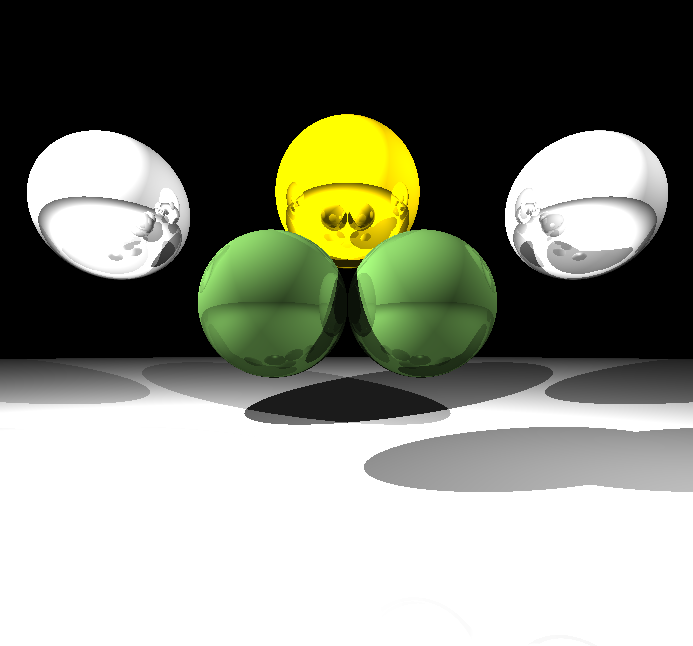
\includegraphics[width=0.62\linewidth,height=0.52\textheight,keepaspectratio]{raytraced_demo.png}
\vfill
{\small April 2026\par}
\end{frame}


\begin{frame}{What is Rendering?}
Rendering takes a scene description as input and produces an image (pixel array) as output.
\vspace{0.5em}
\begin{itemize}
\item Approaches include radiosity, rasterization, and ray tracing.
\item Ray tracing is an \textbf{image-order rendering} method.
\item Each pixel is computed by tracing light-related rays through the scene.
\end{itemize}
\end{frame}


\begin{frame}{Camera to Viewport Rays}
\begin{center}
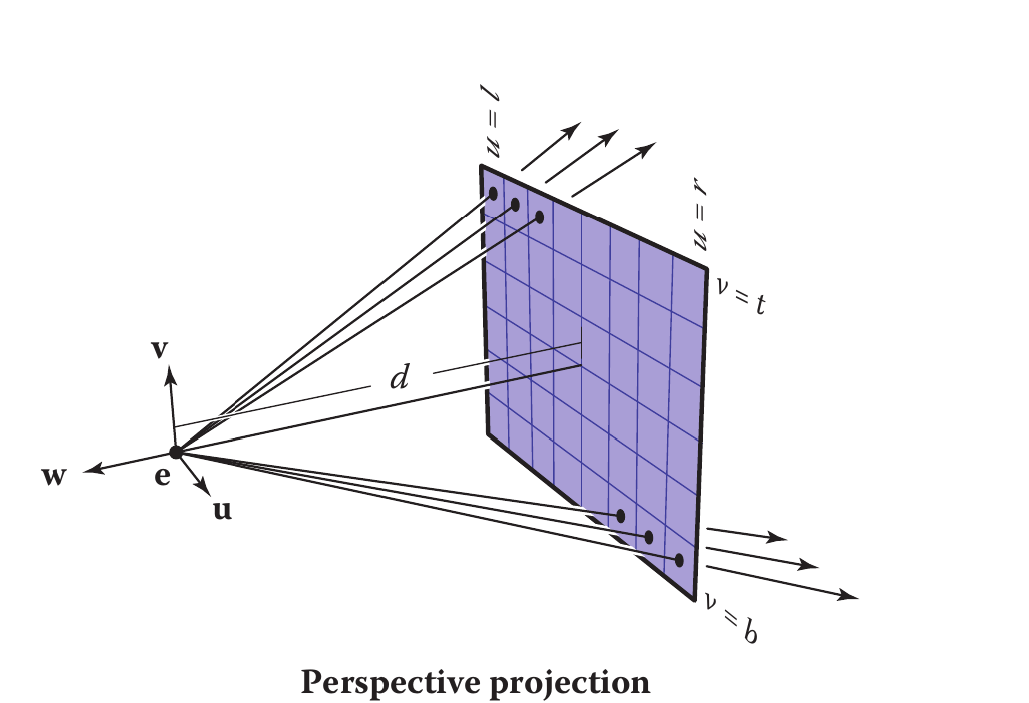
\includegraphics[width=0.82\linewidth,height=0.64\textheight,keepaspectratio]{ray_from_camera_to_screen.png}
\end{center}
\end{frame}

\begin{frame}[fragile]{Basic Structure of a Ray Tracer}
\begin{enumerate}
\item \textbf{Ray Generation}: compute viewing rays from camera geometry.
\item \textbf{Ray Intersection}: find nearest object hit.
\item \textbf{Shading}: compute color from lights, materials, and visibility.
\end{enumerate}
\vspace{0.5em}
Pseudo-code:
\begin{verbatim}
for each pixel do
	compute viewing ray
	if ray hits an object then
		compute surface normal
		evaluate shading model
		set pixel color
	else
		set pixel to background color
\end{verbatim}
\end{frame}

\begin{frame}{Architecture}
\begin{center}
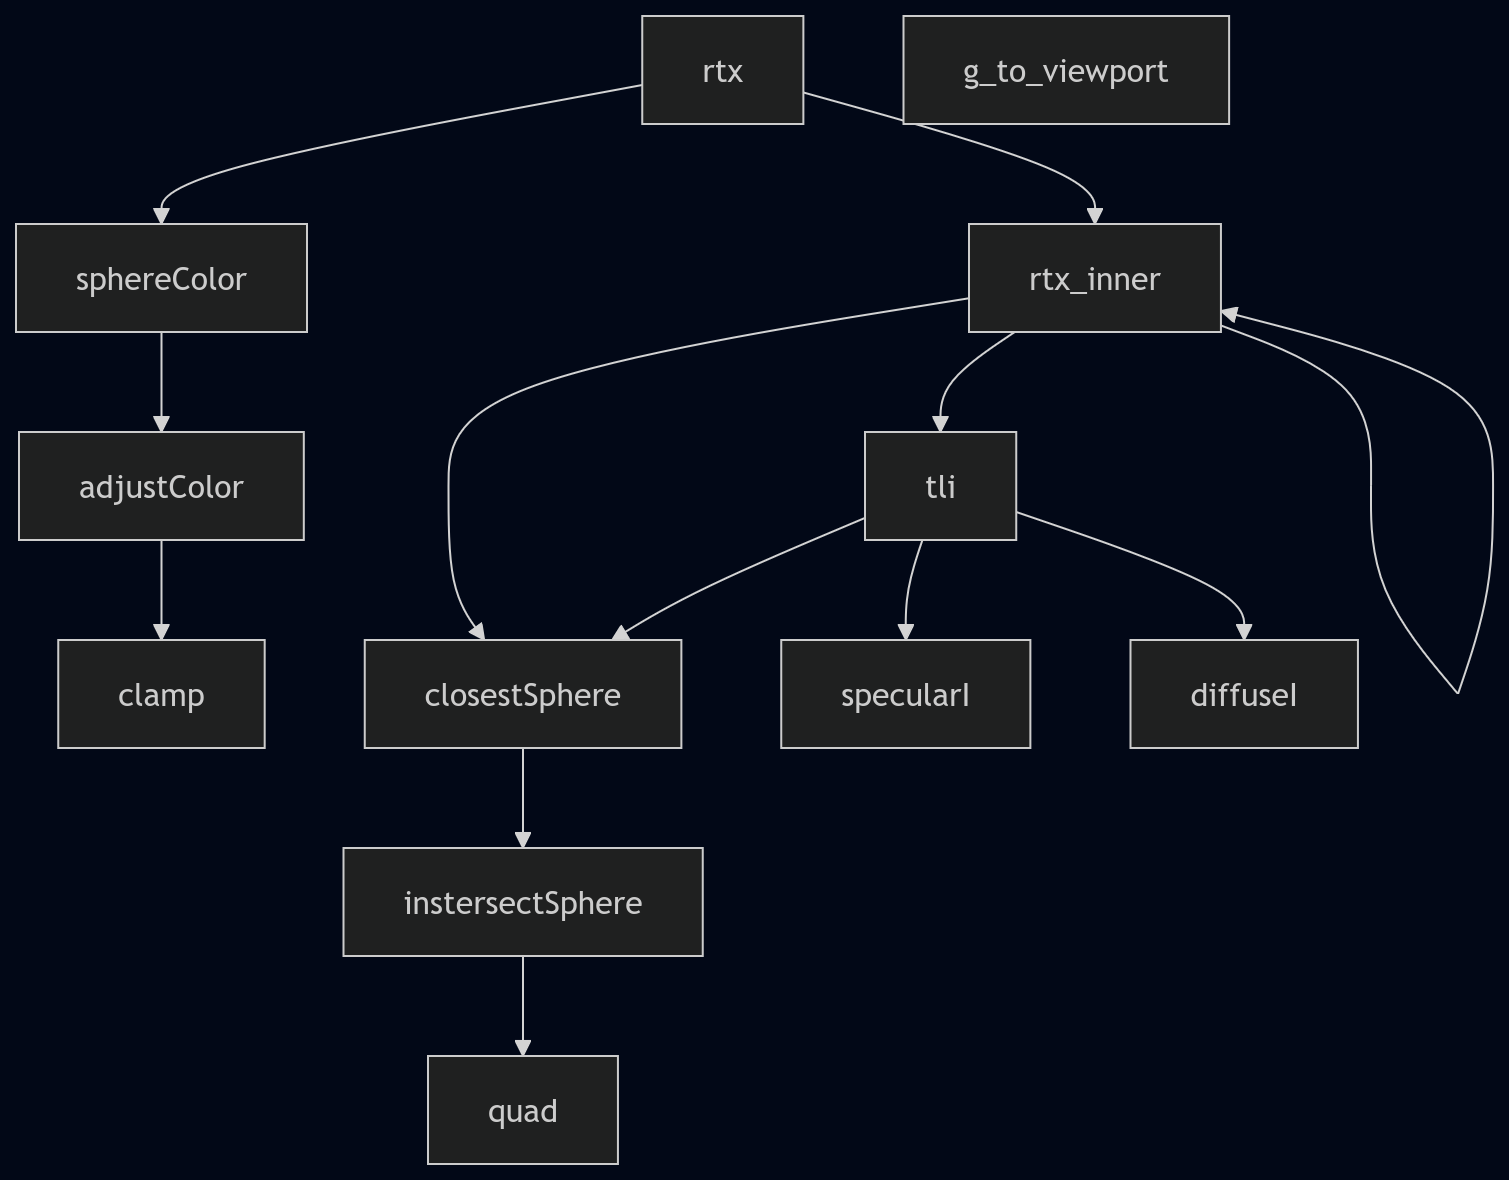
\includegraphics[width=0.88\linewidth,height=0.72\textheight,keepaspectratio]{architecture.png}
\end{center}
\end{frame}

\begin{frame}{Core Helper Functions}
\begin{center}
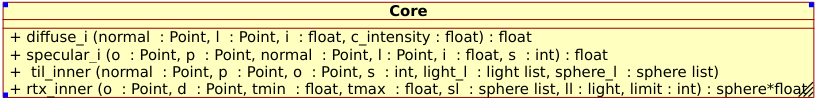
\includegraphics[width=0.88\linewidth,height=0.72\textheight,keepaspectratio]{corediagram.png}
\end{center}
\end{frame}

\begin{frame}{Utility Functions Diagram}
\begin{center}
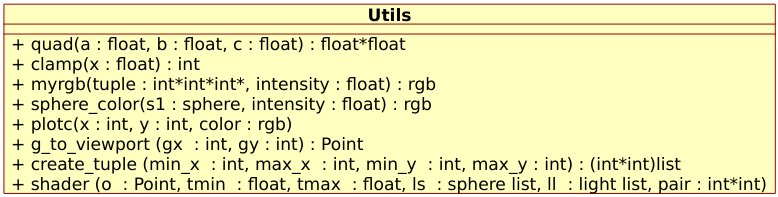
\includegraphics[width=0.88\linewidth,height=0.72\textheight,keepaspectratio]{utilsdiagram.png}
\end{center}
\end{frame}

\begin{frame}{Light Model Diagram}
\begin{center}
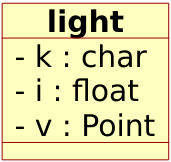
\includegraphics[width=0.88\linewidth,height=0.72\textheight,keepaspectratio]{lightdigram.png}
\end{center}
\end{frame}

\begin{frame}{Point Structure Diagram}
\begin{center}
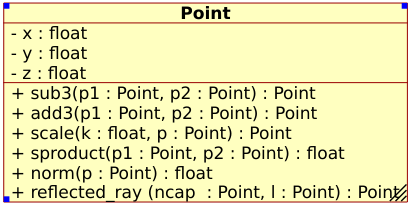
\includegraphics[width=0.88\linewidth,height=0.72\textheight,keepaspectratio]{pointdiagram.png}
\end{center}
\end{frame}

\begin{frame}{Sphere Structure Diagram}
\begin{center}
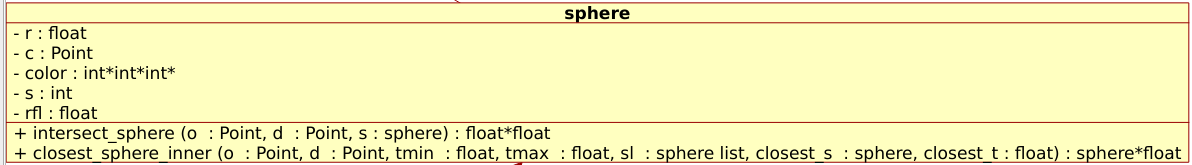
\includegraphics[width=0.88\linewidth,height=0.72\textheight,keepaspectratio]{spherediagram.png}
\end{center}
\end{frame}

\begin{frame}{Color Model (RGB)}
\begin{itemize}
\item Use additive RGB with channel range $[0,255]$.
\item Treat color as a vector $(r,g,b)$.
\item Brightness scaling by $k$: $k(r,g,b)=(kr,kg,kb)$.
\item Clamp each channel to valid bounds after operations.
\end{itemize}
\end{frame}

\begin{frame}{Scene and Camera Setup}
\begin{itemize}
\item Camera at origin $O(0,0,0)$, looking along positive $z$.
\item Viewport in front of camera at distance $d$.
\item Typical setup: $V_w=V_h=d=1$ gives $\text{FOV}\approx53^\circ$.
\item Pixel-to-viewport mapping:
\end{itemize}
\[
V_x = G_x\frac{V_w}{G_w},\quad V_y = G_y\frac{V_h}{G_h},\quad V_z=d
\]
\end{frame}

\begin{frame}{Ray Equation}
Rays from camera through viewport are modeled as:
\[
P = O + t(V-O)
\]
\begin{itemize}
\item $t<0$: behind camera
\item $0\le t\le1$: between camera and viewport
\item $t>1$: in front of viewport
\end{itemize}
\end{frame}

\begin{frame}{Sphere Representation}
Sphere equation:
\[
\langle P-C, P-C \rangle = r^2
\]
\vspace{0.5em}
Data fields used in code:
\begin{itemize}
\item center $C$, radius $r$
\item surface color
\item shininess $s$
\item reflectiveness $rfl \in [0,1]$
\end{itemize}
\end{frame}

\begin{frame}{Ray--Sphere Intersection}
Substitute ray $P=O+t\vec D$ into sphere equation to get:
\[
at^2 + bt + c = 0
\]
where
\[
a=\|\vec D\|^2,\quad b=2\langle \vec D, \vec{CO}\rangle,\quad c=\|\vec{CO}\|^2-r^2
\]
\[
t_{1,2}=\frac{-b\pm\sqrt{b^2-4ac}}{2a}
\]
\end{frame}

\begin{frame}{Ray--Sphere Intersection Geometry}
\begin{center}
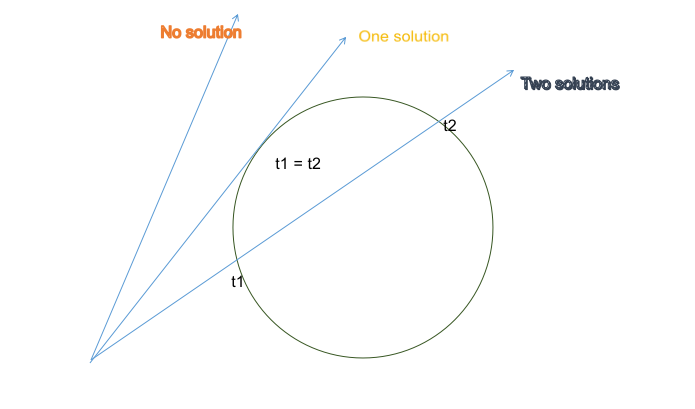
\includegraphics[width=0.76\linewidth,height=0.64\textheight,keepaspectratio]{ray_sphere.png}
\end{center}
\end{frame}

\begin{frame}{Light Types}
\begin{itemize}
\item \textbf{Ambient}: constant scene-wide intensity.
\item \textbf{Point}: position + intensity.
\item \textbf{Directional}: direction + intensity.
\end{itemize}
The workshop uses white lights and sums contributions per point.
\end{frame}

\begin{frame}{Diffuse (Lambertian) Reflection}
Diffuse term for each non-ambient light:
\[
I_{\text{diffuse}} = \sum I_i\max\left(0,\frac{\langle \vec L_i,\vec N\rangle}{\|\vec L_i\|\,\|\vec N\|}\right)
\]
\begin{center}
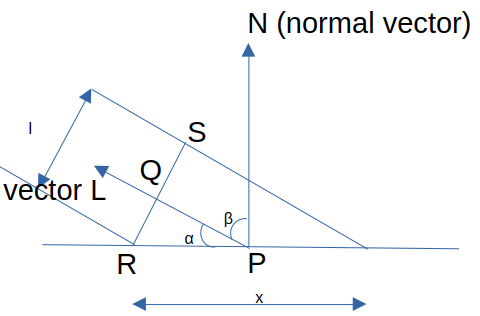
\includegraphics[width=0.58\linewidth]{intensity.png}
\end{center}
\end{frame}

\begin{frame}{Specular Reflection}
Reflection vector:
\[
\vec R = 2\langle\vec L,\hat N\rangle\hat N - \vec L
\]
Specular term:
\[
I_{\text{specular}}=\sum I_i\max\left(0,\frac{\langle\vec R_i,\vec V\rangle}{\|\vec R_i\|\,\|\vec V\|}\right)^s
\]
\begin{center}
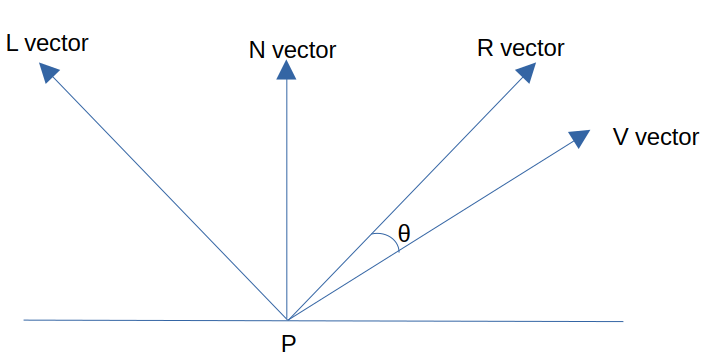
\includegraphics[width=0.58\linewidth]{intensityspecular.png}
\end{center}
\end{frame}

\begin{frame}{Combined Illumination}
\[
I_{\text{total}} = I_a + \sum I_i\left[
\frac{\langle \vec L_i,\vec N\rangle}{\|\vec L_i\|\,\|\vec N\|}
+
\left(\frac{\langle\vec R_i,\vec V\rangle}{\|\vec R_i\|\,\|\vec V\|}\right)^s
\right]
\]
Contributions are accumulated and applied to object color with channel clamping.
\end{frame}

\begin{frame}{Shadow Rays}
To decide if a light contributes at point $P$, trace a secondary ray:
\[
P + t\vec L
\]
\begin{itemize}
\item Point light: check $t\in[\epsilon,1]$.
\item Directional light: check $t\in[\epsilon,\infty)$.
\item If blocked by an object, skip diffuse/specular from that light.
\end{itemize}
\end{frame}

\begin{frame}{Mirror Reflection (Recursive Rays)}
\begin{itemize}
\item At hit point, compute reflected viewing direction.
\item Trace reflected ray recursively.
\item Blend local and reflected colors using reflectiveness $rfl$.
\item Low recursion depths (e.g., 3) often give good visual quality.
\end{itemize}
\end{frame}

\begin{frame}{Experiments}
\begin{enumerate}
\item Change image plane distance $d$.
\item Replace \texttt{double} with \texttt{float}.
\item Vary recursion limit in ray tracing.
\item Change viewport dimensions ($V_w$, $V_h$).
\end{enumerate}
\end{frame}

\begin{frame}{Compilation Commands}
\small
\begin{itemize}
\item Plain build:\\
\texttt{gcc -o render render.c raytracer.c -lm -lSDL3}
\item ASan + debug:\\
\texttt{gcc -g -fsanitize=address -o render3 render3.c raytracer.c -lm -lSDL3}
\item OpenMP:\\
\texttt{gcc -fopenmp -O2 -o render render.c raytracer.c -lm -lSDL3}
\end{itemize}
\end{frame}


\begin{frame}{Further improvements}
\begin{enumerate}
\item Add a scene parser code that reads a json file and loads the scene at runtime. (As opposed to hardcoded scene at compile-time.)
\item Replace \texttt{double} with \texttt{float}.
\item Extend it to other primitives like triangle.
\item Add colored lights, i.e., instead of single intensity, there is different intensity field for each color channel.
\item Add light intensity attenuation.
\item Encapsulate Scene data into single struct.
\end{enumerate}
\end{frame}

\begin{frame}{References}
\small
\begin{thebibliography}{9}
\bibitem{cgpp2013}
John F. Hughes, Andries van Dam, Morgan McGuire, David F. Sklar,
James D. Foley, Steven K. Feiner, and Kurt Akeley.
\newblock \emph{Computer Graphics: Principles and Practice}.
\newblock 3rd edition, 2013.

\bibitem{fcg2015}
Steve Marschner and Peter Shirley.
\newblock \emph{Fundamentals of Computer Graphics}.
\newblock 4th edition, 2015.

\bibitem{cgfs}
Gabriel Gambetta.
\newblock \emph{Computer Graphics from Scratch}.
\newblock No Starch Press, 2021.
\end{thebibliography}
\end{frame}

\begin{frame}[focus]
Questions?
\end{frame}

\end{document}
